\section{Evaluation}
\label{chipper:sec:eval}

\subsection{Application Tail Latency Vs Throughput}
\label{sec:eval-latency}

\begin{figure*}[t]
	\centering

	% Legend
	
\includegraphics[width=.4\linewidth]
	{chipper/figures/overall/overall-chipper-legend.pdf}

	\vspace{-0.5em}

	% =========================================================
	% First row: 5 plots
	% =========================================================
	\subfloat[OpenSearch]{
		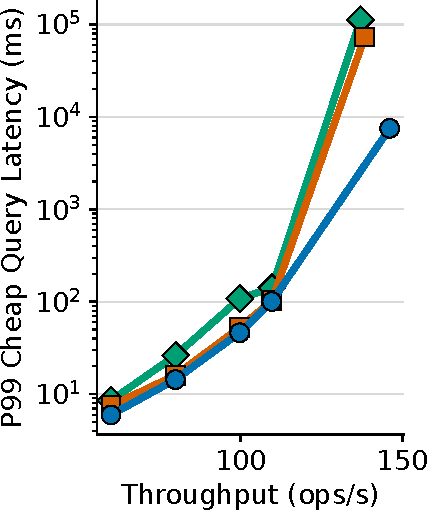
\includegraphics[width=.19\linewidth]
		{chipper/figures/overall/opensearch-chipper-tip-amount.pdf}
		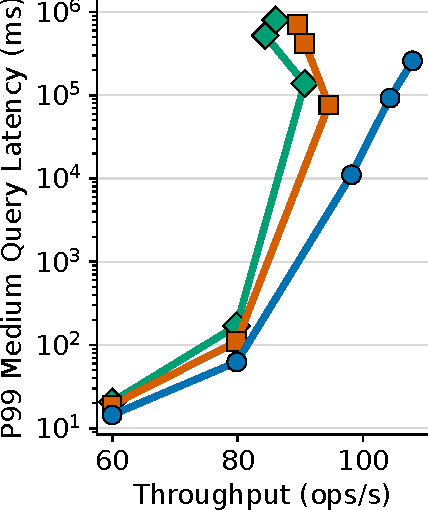
\includegraphics[width=.19\linewidth]
		{chipper/figures/overall/opensearch-chipper-date-histogram-agg.pdf}
		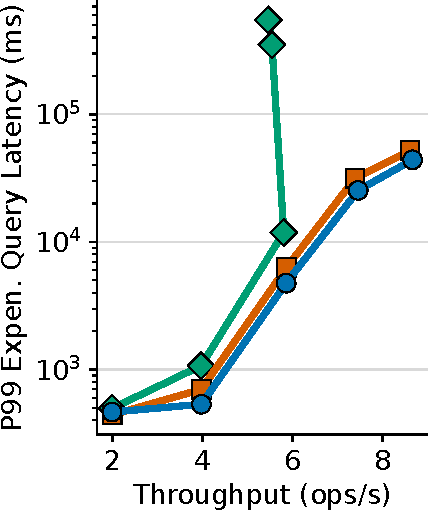
\includegraphics[width=.19\linewidth]
		{chipper/figures/overall/opensearch-chipper-date-histogram-tz.pdf}
	}
	\hspace{-0.8em}
	\subfloat[Lucene]{
		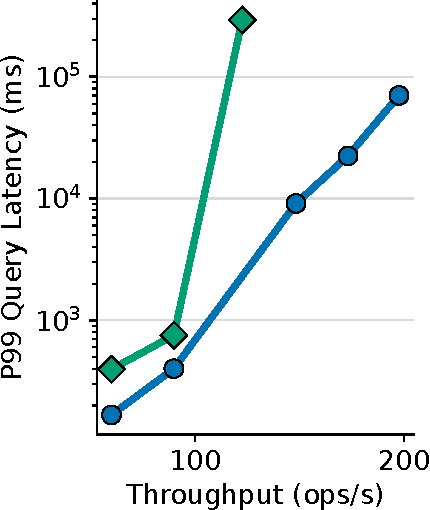
\includegraphics[width=.19\linewidth]
		{chipper/figures/overall/lucene-chipper.pdf}
	}
	\hspace{-0.8em}
	\subfloat[Spark]{
		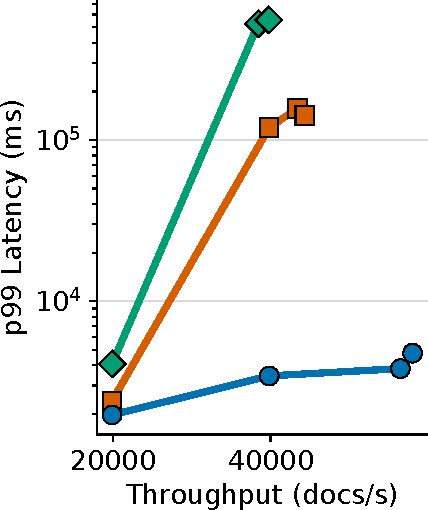
\includegraphics[width=.20\linewidth]
		{chipper/figures/overall/spark-streaming-chipper.pdf}
	}

	\vspace{0.4em}

	% =========================================================
	% Second row: 4 plots
	% =========================================================
	\subfloat[HBase-Workload A]{
		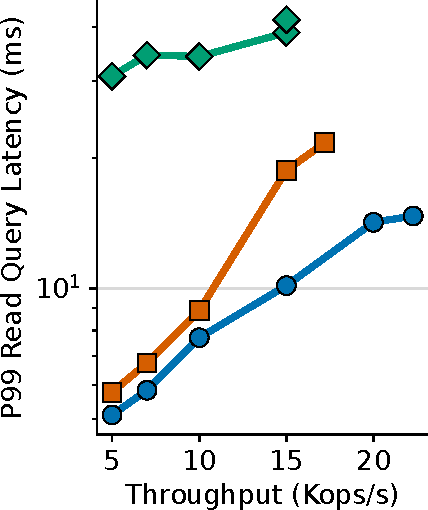
\includegraphics[width=.195\linewidth]
		{chipper/figures/overall/hbase-workloada-chipper-read.pdf}
		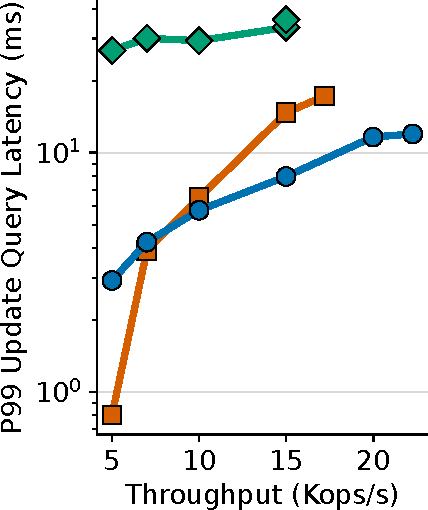
\includegraphics[width=.195\linewidth]
		{chipper/figures/overall/hbase-workloada-chipper-update.pdf}
	}
	\hspace{-0.8em}
	\subfloat[HBase-Workload F]{
		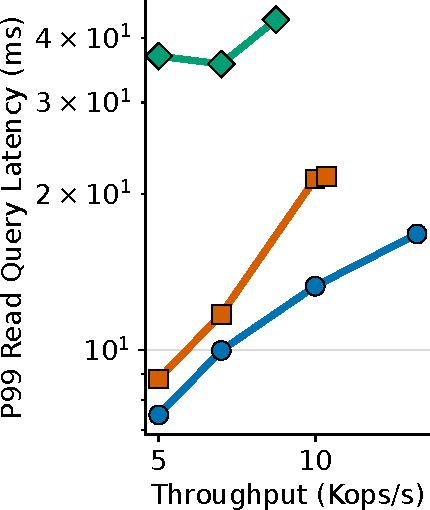
\includegraphics[width=.19\linewidth]
		{chipper/figures/overall/hbase-workloadf-chipper-read.pdf}
		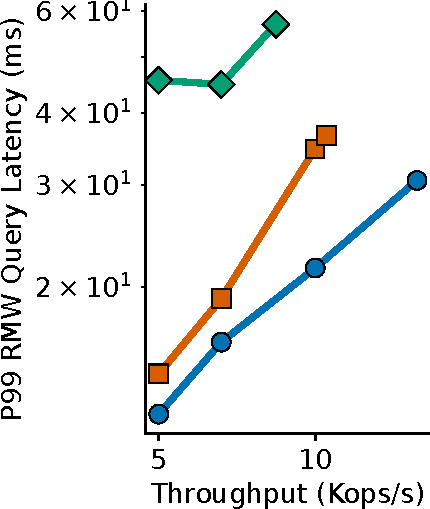
\includegraphics[width=.19\linewidth]
		{chipper/figures/overall/hbase-workloadf-chipper-rmw.pdf}
		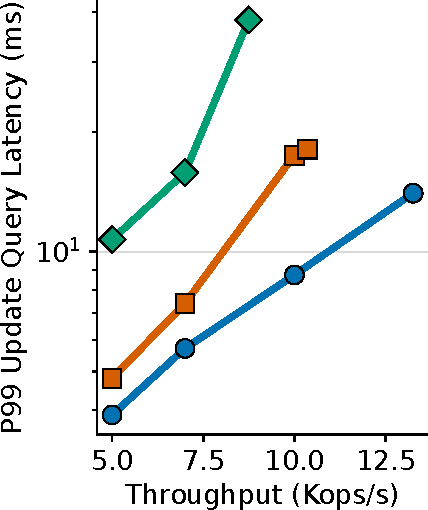
\includegraphics[width=.19\linewidth]
		{chipper/figures/overall/hbase-workloadf-chipper-update.pdf}
	}

	\caption{P99 application latency versus achieved throughput for OpenSearch, Lucene, Spark Streaming, and HBase using on-heap caches, off-heap caches, and \chipperName{}.}
	\label{fig:overall-onheap-offheap-chipper}
\end{figure*}

\paragraph{\textbf{Comparison with on-heap and off-heap caches}}
In this section we evaluate \chipperName{} compared to on-heap and off-heap caching approaches.

Figure~\ref{fig:overall-onheap-offheap-chipper}(a) shows the OpenSearch results, where cheap, medium, and expensive queries run together.
For cheap queries at 110~ops/s, \chipperName{} reduces P99 latency by 29\% over on-heap caching and by 2\% over off-heap caching.
For medium queries at 80~ops/s, \chipperName{} reduces P99 latency by 63\% compared with on-heap caching and by 43\% compared with off-heap caching.
For expensive queries at 6~ops/s, the corresponding reductions are 60\% and 25\%.
The larger gains over on-heap caching come from fewer cache misses: \chipperName{} achieves a 70\% hit rate versus 6\% on-heap, reducing query recomputation.
This matters more as query cost increases.
Compared with off-heap caching, \chipperName{} avoids the S/D cost of accessing cached results while still providing large cache capacity.

Figure~\ref{fig:overall-onheap-offheap-chipper}(b) shows the results for Lucene.
At 90~ops/s, \chipperName{} reduces P99 query latency from 754~ms to 401~ms, a 47\% reduction compared with the on-heap configuration.
As load increases, the on-heap configuration reaches only 123~ops/s before P99 latency increases to 293~s, whereas \chipperName{} continues scaling to 198~ops/s.
At these respective highest measured throughputs, \chipperName{} achieves $1.61\times$ higher throughput while maintaining $4.17\times$ lower P99 latency.
This improvement follows from the larger effective query-cache capacity provided by SH.
\chipperName{} achieves an 88\% cache hit rate, compared with 37\% for the on-heap configuration, reducing query recomputation.

The difference is particularly large for Spark Streaming in Figure~\ref{fig:overall-onheap-offheap-chipper}(c).
At approximately 40K~docs/s, \chipperName{} achieves a P99 latency of 3.4~s, compared with 119.1~s for off-heap caching and 556.0~s for on-heap caching.
Thus, \chipperName{} reduces P99 latency by $34.7\times$ relative to off-heap caching and by $161.8\times$ relative to on-heap caching.
The on-heap configuration suffers from both limited cache capacity and high GC pressure, while the off-heap configuration avoids much of the GC overhead but incurs about 50\% S/D overhead.
By keeping cached RDDs as managed objects in SH, \chipperName{} avoids this S/D overhead while also reducing GC pressure in DH.
\chipperName{} also sustains approximately 58K~docs/s, compared with 44K~docs/s for off-heap caching and 40K~docs/s for on-heap caching, corresponding to approximately $1.31\times$ and $1.46\times$ higher throughput, respectively.

Figures~\ref{fig:overall-onheap-offheap-chipper}(d) and \ref{fig:overall-onheap-offheap-chipper}(e) show the HBase results.
For Workload A at 15K~ops/s, \chipperName{} reduces P99 read latency to 10.2~ms, 46\% lower than off-heap caching and 74--76\% lower than on-heap caching.
For updates, \chipperName{} achieves 8.0~ms P99 latency, reducing latency by 46\% over off-heap caching and 76--78\% over on-heap caching.
\chipperName{} also reaches 22.3K~ops/s, compared with 17.2K~ops/s for off-heap and 15.0K~ops/s for on-heap caching, providing $1.29\times$ and $1.48\times$ higher throughput, respectively.
For Workload F at 10K~ops/s, \chipperName{} reduces P99 latency relative to off-heap caching by 38\% for reads, 38\% for read-modify-write operations, and 50\% for updates.
At 7K~ops/s, where all configurations are directly comparable, \chipperName{} reduces P99 latency relative to on-heap caching by 72\%, 64\%, and 64\% for the same operations.
\chipperName{} reaches 13.3K~ops/s, compared with 10.4K~ops/s for off-heap and 8.7K~ops/s for on-heap caching.
The higher cache hit rate of \chipperName{}, 90\% compared with 60\% on-heap, reduces block-cache misses and the resulting storage accesses.

\begin{figure*}[t]
	\centering

	% Legend
	
\includegraphics[width=.25\linewidth]
	{chipper/figures/overall/overall-tera-vs-chipper-legend.pdf}

	\vspace{-0.5em}

	% =========================================================
	% First row: 5 plots
	% =========================================================
	\subfloat[OpenSearch]{
		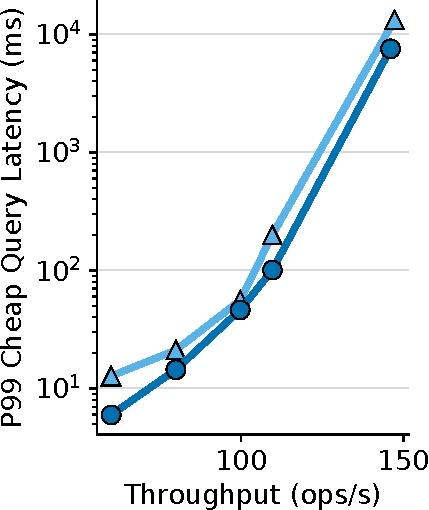
\includegraphics[width=.19\linewidth]
		{chipper/figures/overall/opensearch-tera-vs-chipper-tip-amount.pdf}
		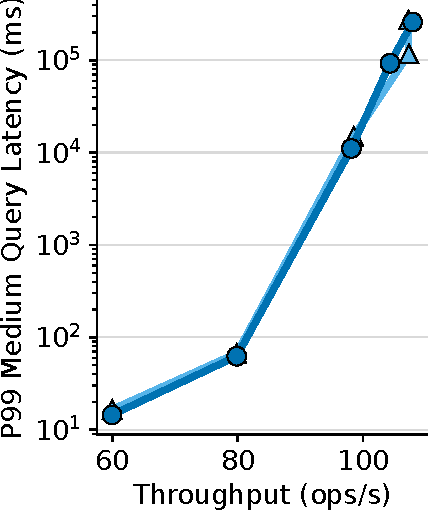
\includegraphics[width=.19\linewidth]
		{chipper/figures/overall/opensearch-tera-vs-chipper-date-histogram-agg.pdf}
		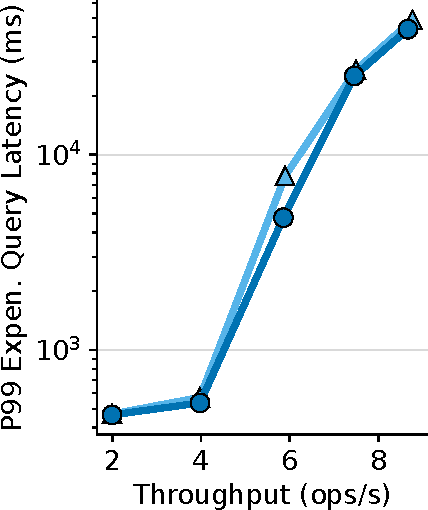
\includegraphics[width=.19\linewidth]
		{chipper/figures/overall/opensearch-tera-vs-chipper-date-histogram-tz.pdf}
	}
	\hspace{-0.8em}
	\subfloat[Lucene]{
		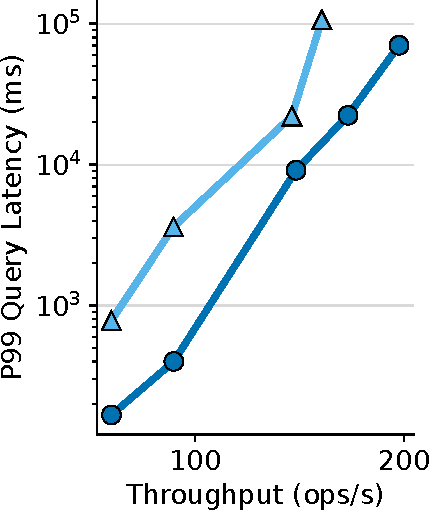
\includegraphics[width=.19\linewidth]
		{chipper/figures/overall/lucene-tera-vs-chipper.pdf}
	}
	\hspace{-0.8em}
	\subfloat[Spark]{
		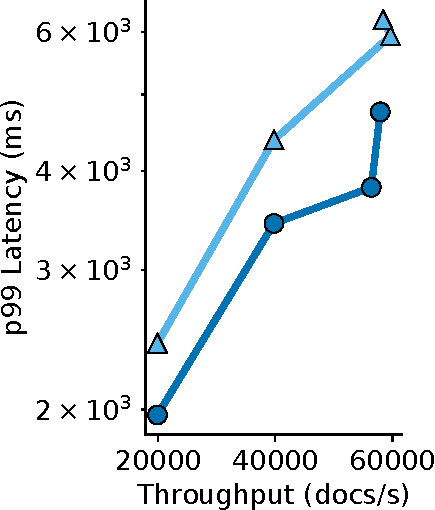
\includegraphics[width=.20\linewidth]
		{chipper/figures/overall/spark-streaming-tera-vs-chipper.pdf}
	}

	\vspace{0.4em}

	% =========================================================
	% Second row: 4 plots
	% =========================================================
	\subfloat[HBase-Workload A]{
		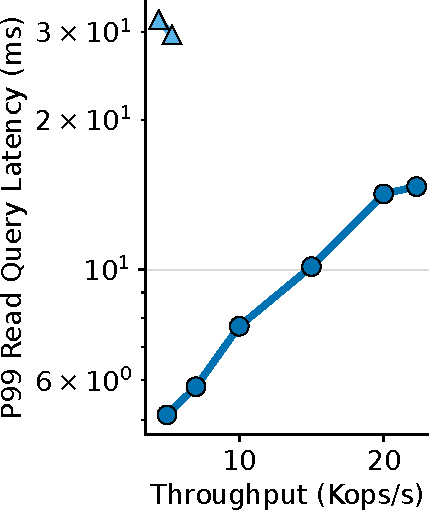
\includegraphics[width=.19\linewidth]
		{chipper/figures/overall/hbase-workloada-tera-vs-chipper-read.pdf}
		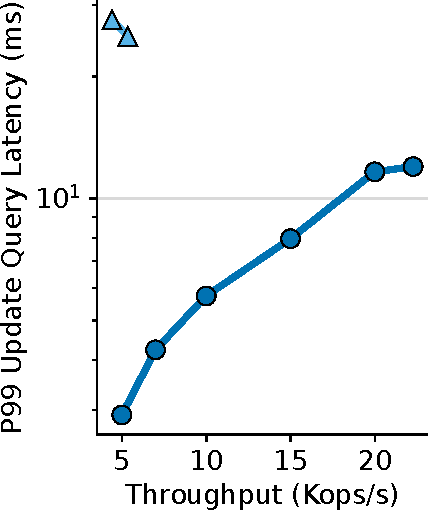
\includegraphics[width=.19\linewidth]
		{chipper/figures/overall/hbase-workloada-tera-vs-chipper-update.pdf}
	}
	\hspace{-0.8em}
	\subfloat[HBase-Workload F]{
		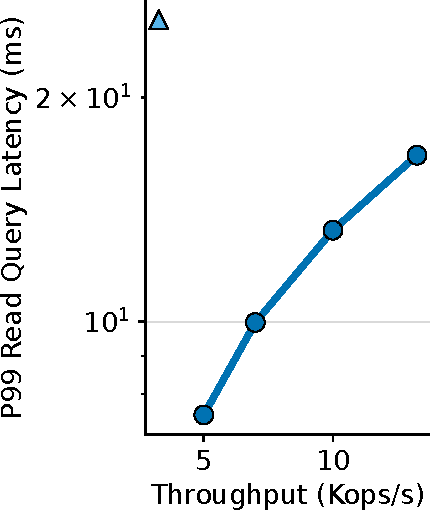
\includegraphics[width=.19\linewidth]
		{chipper/figures/overall/hbase-workloadf-tera-vs-chipper-read.pdf}
		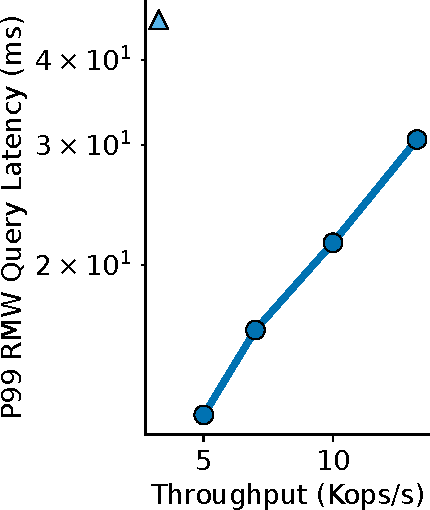
\includegraphics[width=.19\linewidth]
		{chipper/figures/overall/hbase-workloadf-tera-vs-chipper-rmw.pdf}
		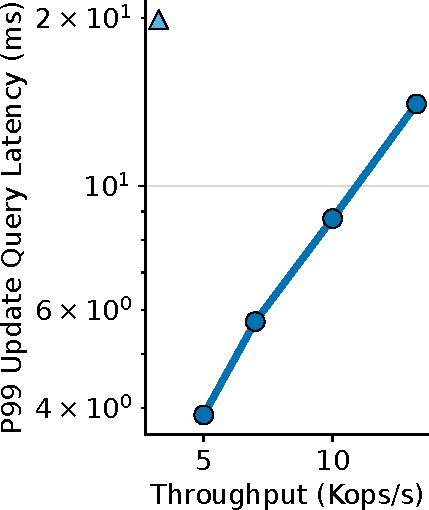
\includegraphics[width=.19\linewidth]
		{chipper/figures/overall/hbase-workloadf-tera-vs-chipper-update.pdf}
	}

	\caption{P99 application latency versus achieved throughput for OpenSearch, Lucene, Spark Streaming, and HBase using TeraHeap and \chipperName{}.}
	\label{fig:overall-tera-vs-chipper}
\end{figure*}

\begin{figure*}[t]
	\centering

	% Legend
	
\includegraphics[width=.25\linewidth]
	{chipper/figures/overall/gc_pauses_legend.pdf}

	\vspace{-0.5em}

	\subfloat[OpenSearch]{
		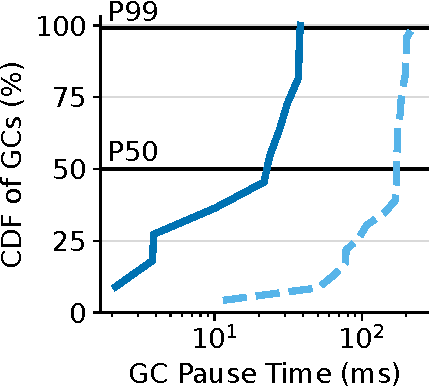
\includegraphics[width=.20\linewidth]
		{chipper/figures/overall/opensearch_gc_pauses_chipper_th_cdf.pdf}
	}
	\subfloat[Spark]{
		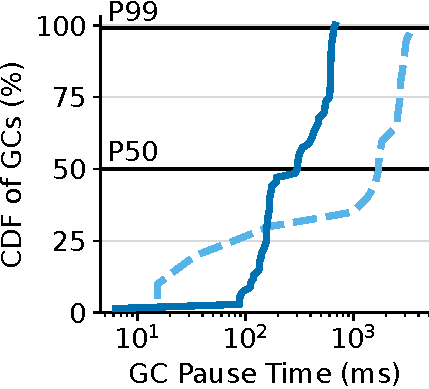
\includegraphics[width=.20\linewidth]
		{chipper/figures/overall/spark_gc_pauses_chipper_th_cdf.pdf}
	}
	\subfloat[HBase-Workload A]{
		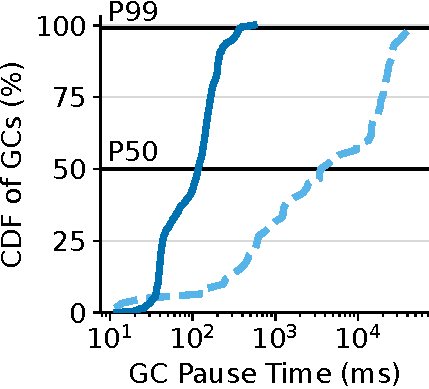
\includegraphics[width=.20\linewidth]
		{chipper/figures/overall/hbase-workloada_gc_pauses_chipper_th_cdf.pdf}
	}
	\subfloat[HBase-Workload F]{
		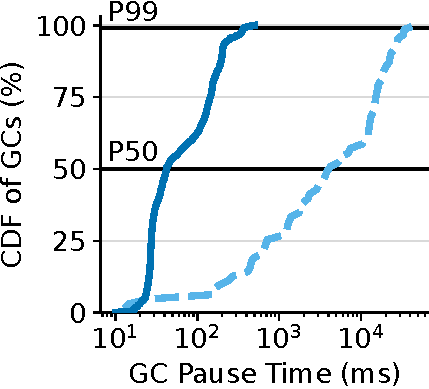
\includegraphics[width=.20\linewidth]
		{chipper/figures/overall/hbase-workloadf_gc_pauses_chipper_th_cdf.pdf}
	}

	\caption{GC pause-time distributions for TeraHeap Full GCs and \chipperName{} Mixed GCs in OpenSearch, Spark Streaming, and HBase Workloads A and F.}
	\label{fig:gc_pauses_chipper_vs_teraheap}
\end{figure*}

\paragraph{\textbf{Comparison with state-of-the-art storage-backed heaps}}
We next compare \chipperName{} with TeraHeap to isolate the benefit of integrating a storage-backed heap with a low-pause collector.
Figure~\ref{fig:overall-tera-vs-chipper} shows the resulting application-level differences.
For OpenSearch, the two systems achieve similar performance because GC activity is low.
For Lucene at 90~ops/s, \chipperName{} achieves $9\times$ lower P99 query latency, reducing it from 3.6~s to 0.4~s, and reaches 198~ops/s compared with 161~ops/s for TeraHeap.
For Spark at 40K~docs/s, \chipperName{} achieves $1.28\times$ lower P99 latency, reducing it from 4.38~s to 3.44~s.
The largest throughput differences occur for HBase, where \chipperName{} reaches 22.3~Kops/s versus 5.4~Kops/s for Workload A and 13.3~Kops/s versus 3.3~Kops/s for Workload F, providing $4.2\times$ and $4.1\times$ higher throughput, respectively.

Figure~\ref{fig:gc_pauses_chipper_vs_teraheap} explains these application-level differences through the corresponding GC pause distributions.
For OpenSearch, \chipperName{} reduces the P99 GC pause from 221~ms to 38~ms, but the small number of collections limits their impact on application latency.
For Spark, \chipperName{} reduces the median GC pause from 1.72~s to 303~ms and the P99 from 3.54~s to 659~ms, both by more than $5\times$.
The difference is larger for HBase.
For Workload A, \chipperName{} reduces the median GC pause from 3.90~s to 117~ms and the P99 from 43.8~s to 374~ms, corresponding to $33\times$ and $117\times$ reductions.
For Workload F, the corresponding reductions are from 4.23~s to 42~ms at the median and from 37.7~s to 370~ms at P99, over $100\times$ in both cases.

\subsection{Effectiveness of SH-Aware Region Ranking}
\label{sec:eval-selection}

\begin{figure}[h]
	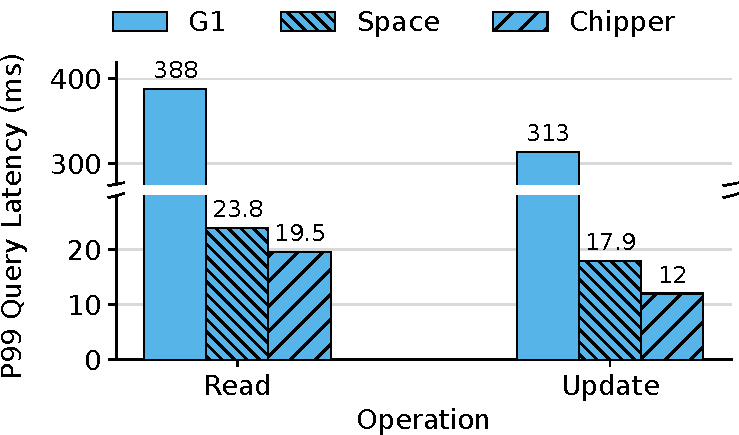
\includegraphics[width=.4\linewidth]{chipper/figures/eval/model/p99_query.pdf}
	\caption{P99 query latency for read and update operations in HBase Workload A under the three region-efficiency models used to rank candidate regions for collection.}
	\label{fig:model-p99}
\end{figure}

We evaluate how effectively \chipperName{}'s SH-aware region-efficiency model ranks candidate regions for collection and how this choice affects application tail latency.
We compare three region-efficiency models while keeping the rest of the system unchanged.
The G1 model uses G1's original region efficiency, which considers garbage reclaimed from a region and the predicted cost of evacuating its live objects within DH.
The Space model additionally accounts for the DH space reclaimed when live SH-candidate objects are evacuated to SH, without considering their evacuation overhead.
The \chipperName{} model accounts for both the additional DH space reclaimed through evacuation to SH and the higher evacuation cost of SH-bound objects.

Figure~\ref{fig:model-p99} shows the resulting P99 query latency for HBase Workload A.
For read operations, \chipperName{} achieves $19.9\times$ lower P99 latency than the G1 model and $1.22\times$ lower P99 latency than the Space model, while for update operations the corresponding improvements are $26.1\times$ and $1.49\times$.
Table~\ref{tab:model-gc} shows that these application-level differences follow from substantially different GC behavior.
The G1 model triggers 89 Full GCs, whereas neither the Space model nor the \chipperName{} model triggers a Full GC.
Compared with the G1 model, Table~\ref{tab:model-gc} shows that \chipperName{} reduces total Mixed GC time by $14.1\times$, the median Mixed GC pause by $3.7\times$, the P90 by $7.3\times$, the P99 by $5.6\times$, and the maximum pause by $5.9\times$.
Compared with the Space model, Table~\ref{tab:model-gc} shows that \chipperName{} performs 34 more Mixed GCs but still reduces total Mixed GC time by $1.09\times$, the median pause by $1.50\times$, the P90 by $1.16\times$, and the maximum pause by $1.93\times$.
The P99 Mixed GC pause is similar for the Space and \chipperName{} models, differing by only $1.02\times$.

\begin{table*}[h]
	\setlength{\aboverulesep}{0pt}
	\setlength{\belowrulesep}{0pt}
	\centering
	\small
	\setlength{\tabcolsep}{4pt}
	\renewcommand{\arraystretch}{1.05}
	\caption{GC statistics for the three region-efficiency models used to rank candidate regions for collection for HBase Workload A.}
	\label{tab:model-gc}
	\begin{tabular}{l|cc|ccccccc}
		\toprule
		\multirow{2}{*}{\textbf{Model}}
		 & \multicolumn{2}{c|}{\textbf{Full GC}}
		 & \multicolumn{7}{c}{\textbf{Mixed GC}} \\
		\cline{2-10}
		\noalign{\vskip 2pt}
		 & \textbf{\#}
		 & \shortstack{\textbf{Time}             \\ \textbf{(s)}}
		 & \textbf{\#}
		 & \shortstack{\textbf{Time}             \\ \textbf{(s)}}
		 & \shortstack{\textbf{Min}              \\ \textbf{(ms)}}
		 & \shortstack{\textbf{Max}              \\ \textbf{(ms)}}
		 & \shortstack{\textbf{P50}              \\ \textbf{(ms)}}
		 & \shortstack{\textbf{P90}              \\ \textbf{(ms)}}
		 & \shortstack{\textbf{P99}              \\ \textbf{(ms)}} \\
		\midrule
		G1
		 & 89
		 & 21.84
		 & 721
		 & 568.81
		 & 21.14
		 & 3077.35
		 & 480.89
		 & 2362.05
		 & 2835.51                               \\

		Space
		 & 0
		 & 0
		 & 215
		 & 44.16
		 & 25.86
		 & 1008.50
		 & 195.37
		 & 374.57
		 & 522.63                                \\

		\chipperName{}
		 & 0
		 & 0
		 & 249
		 & 40.36
		 & 19.35
		 & 521.87
		 & 130.05
		 & 322.14
		 & 510.53                                \\
		\bottomrule
	\end{tabular}
\end{table*}

\begin{figure*}[h]
	\subfloat[G1 model]{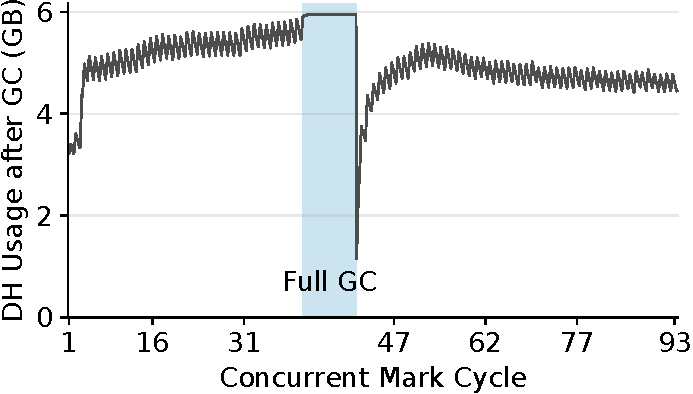
\includegraphics[width=0.325\linewidth]{chipper/figures/eval/model/g1_model_evac.pdf}}
	\subfloat[Space model]{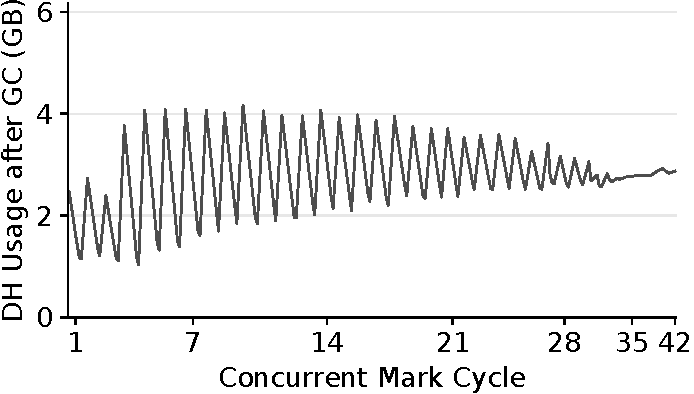
\includegraphics[width=0.325\linewidth]{chipper/figures/eval/model/space_model_evac.pdf}}
	\subfloat[\chipperName{} model]{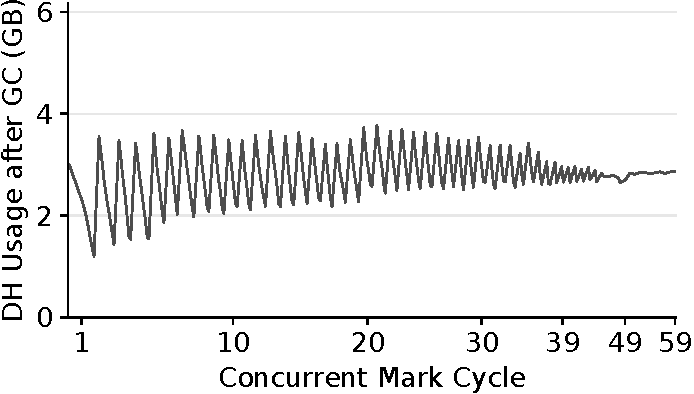
\includegraphics[width=0.325\linewidth]{chipper/figures/eval/model/cost_model_evac.pdf}}
	\caption{DH heap usage after Mixed and Full GCs for HBase Workload A under the three region-efficiency models used to rank candidate regions for collection.
		The x-axis denotes concurrent-mark cycles, each of which include multiple Mixed GCs.}
	\label{fig:model-heap}
\end{figure*}

Figure~\ref{fig:model-heap} shows why the G1 model triggers Full GCs.
Before the Full-GC sequence, Mixed GCs repeatedly collect regions but leave DH close to capacity.
The G1 model ranks regions using only the garbage reclaimed from the selected region and therefore does not account for the additional DH space reclaimed when live SH-candidate objects are moved to SH.
As a result, its Mixed GCs do not reclaim DH quickly enough to prevent memory pressure from reaching the Full-GC path.

The repeated Full GCs are amplified by G1's skip-compaction optimization.
During Full GC, G1 avoids compacting regions with less than 5\% garbage.
This optimization is normally useful because compacting nearly full regions provides little space benefit.
In this workload, however, some of these skipped regions contain live SH-candidate large objects.
Since large objects are migrated to SH through the Full-GC path, skipping these regions also postpones their migration.
Consequently, a Full GC can finish without reclaiming enough DH space, and another Full GC follows shortly afterwards.
For example, near the end of this sequence, one Full GC scans only 17 regions while skipping 1,355 regions.
The final Full GC instead scans 1,363 regions and skips only 9, allowing the remaining large SH candidates to be migrated.
The final Full GC migrates \SI{1.72}{GB} to SH, explaining the drop in DH usage in Figure~\ref{fig:model-heap}(a).

This large-object migration also explains the long Mixed GC pauses that follow.
The migrated large objects are subsequently updated by the application, creating backward references from SH to newly allocated objects in DH.
Before the final Full GC, the run has no backward references.
Immediately after the migration, the first Mixed GC processes 283,179 backward references and spends \SI{228.990}{ms} scanning the SH card table.
As execution continues, this cost becomes the dominant component of the longest Mixed GC pauses.
For the Mixed GC with the maximum pause, the collector processes 173,761 backward references and spends \SI{3021.291}{ms} scanning the SH card table.
This accounts for \SI{3021.291}{ms} of its \SI{3077.35}{ms} pause.
The Space and \chipperName{} models avoid this behavior because they reclaim sufficient DH space during Mixed GCs and therefore do not trigger the Full-GC migration of these large objects.
Their runs consequently have no backward references from these objects.

\begin{figure*}[h]
	% Legend
	
\includegraphics[width=.4\linewidth]{chipper/figures/eval/model/cost_model_evac_cycle13_legend.pdf}
	\\
	\subfloat[G1 model]{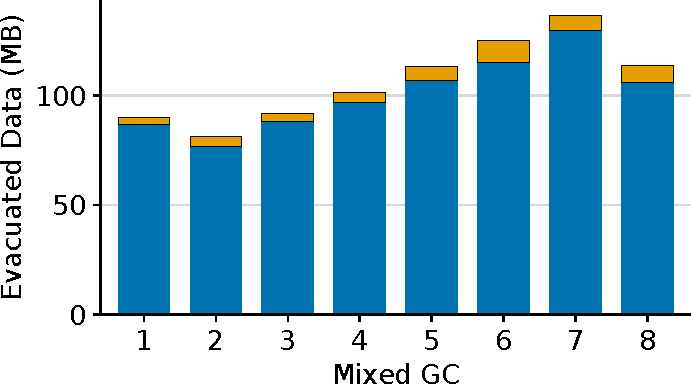
\includegraphics[width=0.325\linewidth]{chipper/figures/eval/model/g1_model_evac_cycle40.pdf}}
	\subfloat[Space model]{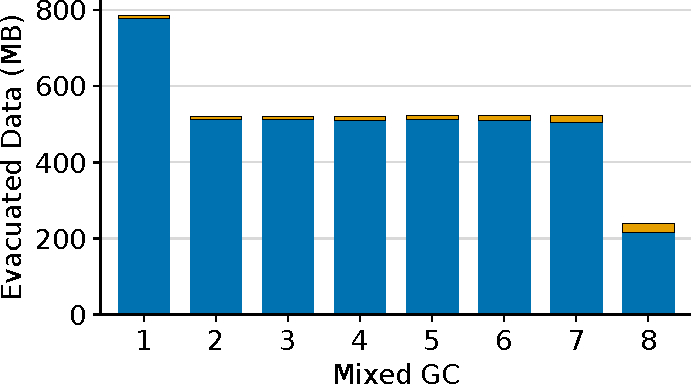
\includegraphics[width=0.325\linewidth]{chipper/figures/eval/model/space_model_evac_cycle4.pdf}}
	\subfloat[\chipperName{} model]{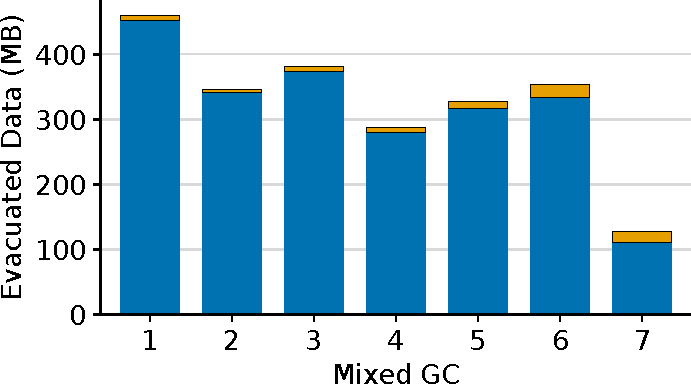
\includegraphics[width=0.325\linewidth]{chipper/figures/eval/model/cost_model_evac_cycle13.pdf}}
	\caption{Data evacuated to DH and SH by individual Mixed GCs within one concurrent-mark cycle for HBase Workload A under the three region-efficiency models, where (a) shows the G1 model in the concurrent-mark cycle immediately before the Full GC, (b) shows the Space model in the concurrent-mark cycle containing its maximum Mixed GC pause of \SI{1008.5}{ms}, and (c) shows the \chipperName{} model in the concurrent-mark cycle containing its maximum Mixed GC pause of \SI{521.87}{ms}.}
	\label{fig:model-evacuation}
\end{figure*}

Figure~\ref{fig:model-evacuation} isolates the remaining difference between the Space and \chipperName{} models.
For the G1 model, we show the concurrent-mark cycle immediately before the Full-GC sequence.
Its eight Mixed GCs evacuate only about \SI{806}{MB} to SH in total, which is insufficient to prevent DH from reaching the Full-GC path.
For the Space and \chipperName{} models, we show the concurrent-mark cycles containing their maximum Mixed GC pauses.
The Space model evacuates \SI{4055}{MB} to SH in this cycle, whereas \chipperName{} evacuates \SI{2207}{MB}, a difference of \SI{1848}{MB}.
The Space model credits SH-bound live bytes as reclaimed DH space but does not account for their higher SH evacuation cost.
It therefore assigns overly high efficiency to regions with large amounts of SH-bound live data and can place too much SH evacuation work in the same Mixed GC cycle.
The \chipperName{} model includes the SH evacuation cost in the region-efficiency calculation, reducing the amount of expensive SH evacuation selected together.
This difference reduces the maximum Mixed GC pause from \SI{1008.50}{ms} with the Space model to \SI{521.87}{ms} with \chipperName{}, while still reclaiming enough DH space to avoid Full GC.

\subsection{Impact of SH Allocation-Lock Granularity}
\label{sec:eval-scalability}

We evaluate how SH allocation-lock granularity affects Mixed GC performance and application tail latency.
As a baseline, we use a single global allocation lock, which serializes SH destination reservation and updates to the shared SH allocation metadata.
We compare this baseline with \chipperName{}'s per-region allocation locks, which allow GC threads targeting different SH regions to reserve destinations concurrently.

We evaluate all four applications, but report Lucene and Spark in Table~\ref{tab:allocation-locks} because they expose allocation-lock contention.
HBase and OpenSearch evacuate only a few thousand objects per Mixed GC, and these objects are relatively large.
They therefore perform fewer SH allocation operations and acquire the allocation lock less frequently.
As a result, the global and per-region implementations have similar Mixed GC pause distributions and application P99 latency for HBase and OpenSearch, so we omit them for brevity.

\begin{table*}[h]
	\centering
	\small
	\setlength{\tabcolsep}{3.5pt}
	\renewcommand{\arraystretch}{1.05}

	\caption{Impact of SH allocation-lock granularity on application P99 latency, Mixed GC time and pause distribution, and SH filler space overhead from duplicate evacuation reservations.}
	\label{tab:allocation-locks}

	\begin{tabular}{@{}cccccccccc@{}}
		\toprule

		\multirow[c]{2}{*}[-0.6ex]{\textbf{Application}}
		 &
		\multirow[c]{2}{*}{\textbf{\shortstack[c]{Lock      \\ granularity}}}
		 &
		\multirow[c]{2}{*}{\textbf{\shortstack[c]{P99 query \\ latency (ms)}}}
		 &
		\multicolumn{6}{c}{\textbf{Mixed GC}}
		 &
		\multirow[c]{2}{*}{\textbf{\shortstack[c]{Filler    \\space (\%)}}}
		\\

		\cmidrule(lr){4-9}

		 &
		 &
		 &
		\textbf{\#}
		 &
		\textbf{\shortstack[c]{Time                         \\(s)}}
		 &
		\textbf{\shortstack[c]{P50                          \\(ms)}}
		 &
		\textbf{\shortstack[c]{P95                          \\(ms)}}
		 &
		\textbf{\shortstack[c]{P99                          \\(ms)}}
		 &
		\textbf{\shortstack[c]{Max                          \\(ms)}}
		 &
		\\

		\midrule

		\multirow{2}{*}{Lucene}
		 & Global
		 & 5.5
		 & 83
		 & 5.8
		 & 64.89
		 & 140.35
		 & 206.64
		 & 227.41
		 & 0.00
		\\

		 & Per-region
		 & 1.7
		 & 15
		 & 1.1
		 & 69.10
		 & 124.26
		 & 166.27
		 & 166.29
		 & 0.20
		\\

		\midrule

		\multirow{2}{*}{Spark}
		 & Global
		 & 87
		 & 321
		 & 115.9
		 & 345.97
		 & 921.32
		 & 1022.48
		 & 1082.11
		 & 0.00
		\\

		 & Per-region
		 & 3.1
		 & 68
		 & 23
		 & 304.19
		 & 641.09
		 & 652.21
		 & 673.90
		 & 0.17
		\\

		\bottomrule
	\end{tabular}
\end{table*}


Table~\ref{tab:allocation-locks} shows that per-region locking substantially reduces Mixed GC time.
For Lucene, total Mixed GC time decreases from 5.8~s to 1.1~s, an 81\% reduction.
For Spark, it decreases from 115.9~s to 23.0~s, an 80\% reduction.
The number of Mixed GCs also decreases from 83 to 15 for Lucene and from 321 to 68 for Spark.

Per-region locking also reduces Mixed GC pause times, especially at the tail.
For Lucene, P50 increases slightly from 64.9~ms to 69.1~ms, while P95, P99, and the maximum pause decrease by 11\%, 20\%, and 27\%, respectively.
For Spark, P50, P95, P99, and the maximum pause decrease by 12\%, 30\%, 36\%, and 38\%, respectively.
These results show that the global lock limits evacuation parallelism when GC threads frequently reserve destinations in SH, whereas per-region locks allow reservations to proceed in parallel across different SH regions.

The reduction in Mixed GC time and pause times translates to lower application tail latency.
For Lucene, P99 query latency decreases from 5.5~ms to 1.7~ms, a 69\% reduction.
For Spark, P99 query latency decreases from 87.0~ms to 3.1~ms, a 96\% reduction.

Per-region locking introduces little additional SH space overhead from duplicate evacuation reservations.
SH filler objects occupy only 0.20\% of allocated SH space for Lucene and 0.17\% for Spark.
Thus, per-region allocation locks preserve parallel SH evacuation while adding negligible filler-space overhead.

\subsection{DH Space Reclaimed from Large Objects}
\label{sec:eval-large}

To evaluate the impact of placing large-object migration on the incremental-GC path, we compare two Lucene configurations.
In the first, we increase the G1 region size from its \SI{4}{MB} default for this heap size to \SI{16}{MB}, causing the large Lucene objects in this experiment to fall below G1's humongous-object threshold and therefore become eligible for regular evacuation to SH during Mixed GCs.
In the second, we use the default \SI{4}{MB} regions, under which these objects are humongous and \chipperName{} defers their migration to Full GC using the collector's existing mechanism for relieving memory pressure.
We use the larger region size as an experimental mechanism to place these objects on the Mixed GC evacuation path.

\begin{figure*}[h]
	\centering
	\subfloat[Query tail latency and throughput]{
		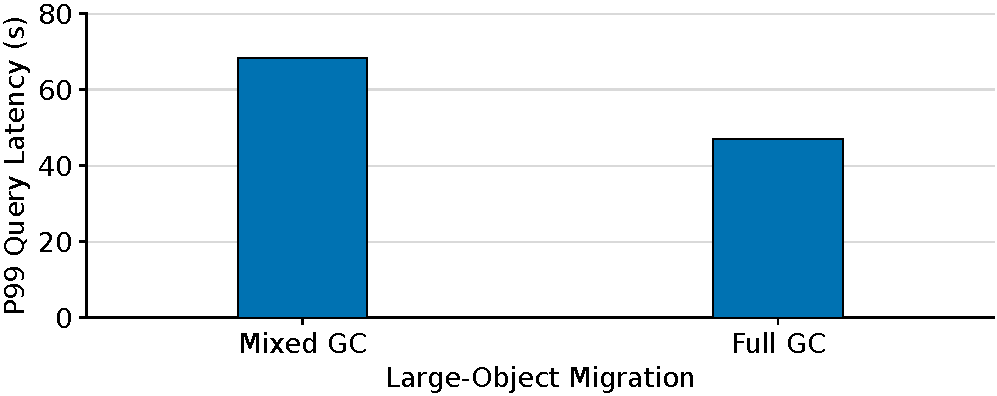
\includegraphics[width=0.48\linewidth]
		{chipper/figures/eval/humongous/lucene_large_object_performance.pdf}
	}
	\hfill
	\subfloat[Distribution of Mixed GC pauses]{
		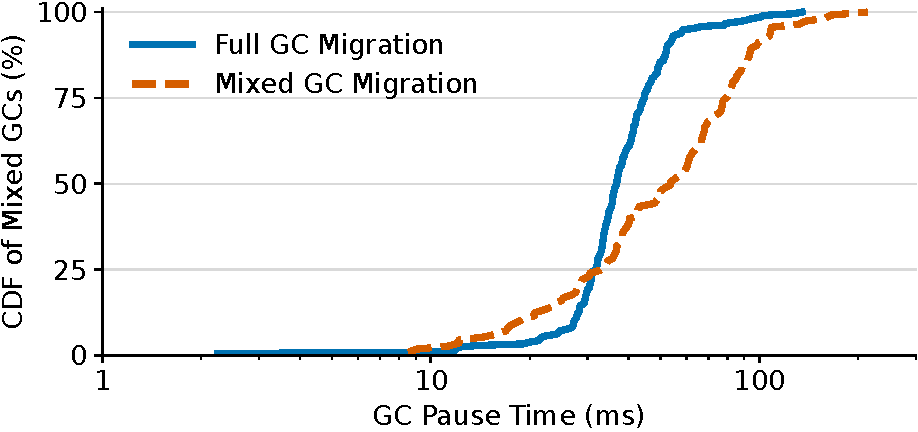
\includegraphics[width=0.48\linewidth]
		{chipper/figures/eval/humongous/gc_pauses_cdf.py.pdf}
	}

	\caption{
		Impact of large-object migration strategy on Lucene.
		(a) Achieved throughput and P99 query latency when large objects are migrated during Mixed GCs or Full GCs.
		(b) Distribution of Mixed GC pause times for the two migration strategies.	}
	\label{fig:humongous}

\end{figure*}

Figure~\ref{fig:humongous}(a) shows that deferring large-object migration to Full GC improves application performance.
At a target throughput of 200~ops/s, Full-GC migration achieves 182.68~ops/s, compared with 172.72~ops/s when large objects are migrated during Mixed GCs, a 5.8\% improvement.
Full-GC migration also reduces P99 query latency from 68.3~s to 47.0~s, a 31.2\% reduction.

Figure~\ref{fig:humongous}(b) explains this improvement.
Migrating large objects during Mixed GCs adds their copy cost to latency-critical incremental collections, shifting the Mixed GC pause distribution toward longer pauses and producing a heavier tail.
Deferring this work to Full GC removes large-object copying from the Mixed GC evacuation path, shifting the distribution toward shorter pauses.
Consequently, Mixed GCs perform only the regular evacuation work for which the incremental collector is designed, while large-object migration is performed on the less frequent memory-pressure-relief path.
The shorter Mixed GC pauses reduce interference with application execution, which leads to both higher achieved throughput and lower P99 query latency.
